%%%%%%%%%%%%%%%%%%%%%%%%%%%%%%%%%%%%%%%%%%%%%%%%%%%%%%%%%%%%%%%%%%%%%%%%%%%%%%%%
%%  Article LaTeX style, by Anthony Wharton
\documentclass[11pt,twocolumn,a4paper]{article}
\usepackage[backend=bibtex,style=numeric-comp,sorting=none]{biblatex}
\usepackage[compact]{titlesec}
\usepackage{geometry}
\usepackage{lipsum}
\usepackage{listings}
\usepackage{graphicx}
\usepackage{xspace}
\usepackage{textcomp}
\usepackage{array}
\usepackage{caption}
\usepackage{titling}
\usepackage{calc}
\usepackage{setspace}
\usepackage{changepage}

%%%%%%%%%%%%%%%%%%%%%%%%%%%%%%%%%%%%%%%%%%%%%%%%%%%%%%%%%%%%%%%%%%%%%%%%%%%%%%%%
%%  Package Setup

% Set up borders and column separation
\setlength{\columnsep}{0.7cm}
\geometry{left=1.2cm,right=1.2cm,top=1cm,bottom=1.2cm}

% Set up title spacing
% \titlespacing{command}{left spacing}{before spacing}{after spacing}[right]
\titlespacing\section{0pt}{1pt}{1pt}
\titlespacing\subsection{0pt}{1pt}{1pt}
\titlespacing\subsubsection{0pt}{1pt}{1pt}


% Set up paragraph spacing and enforce hyphenation penalty
\setlength{\parindent}{0.7em}
\setlength{\parskip}{0.5em}
\setlength{\textfloatsep}{0.25cm}
\setlength{\droptitle}{-1.3cm}
\setlength{\footskip}{\paperheight
    -(2cm+\voffset+\topmargin+\headheight+\headsep+\textheight)
    -1.2cm}
\hyphenpenalty 500

% Set up figure/table captions
% \DeclareCaptionLabelSeparator{emdash}{\textemdash}
\DeclareCaptionFont{mysize}{\fontsize{9}{9.6}\selectfont}
\captionsetup{font=mysize,justification=centering}

% Set up bibliography
\bibliography{references}
\renewcommand*{\bibfont}{\small}

% Set up more intelligent trademark symbol with spacing
% \let\OldTexttrademark\texttrademark
% \renewcommand{\texttrademark}{\OldTexttrademark\xspace}
\def\tm{\texttrademark\xspace}

% Set up code appropriate code listing appearance.
\lstset{
    basicstyle=\footnotesize,
    % numbers=left,
    % numberstyle=\tiny,
    xleftmargin=1.2em,
    columns=flexible,
    linewidth=\columnwidth,
    breaklines=true,
    captionpos=b,
    escapeinside=\!\!,
    language=C,
    literate={->}{$\rightarrow{}$}{1}
             {=>}{$\Rightarrow{}$}{1},
    moredelim=[is][\ttfamily\kern-0.1ex\textsubscript]{^}{\ },
    morekeywords={}
}

% \begin{lstlisting}[gobble=8, caption="A sample code listing.", label=lst1]

\begin{document}
%%%%%%%%%%%%%%%%%%%%%%%%%%%%%%%%%%%%%%%%%%%%%%%%%%%%%%%%%%%%%%%%%%%%%%%%%%%%%%%%
%%  Title
\title{\LARGE\bfseries Exploring Jacobi Method Parallelism}
\date{\vspace{-1cm}} % No date
\author{Anthony Wharton \\ aw15885@bristol.ac.uk}
\maketitle

%%%%%%%%%%%%%%%%%%%%%%%%%%%%%%%%%%%%%%%%%%%%%%%%%%%%%%%%%%%%%%%%%%%%%%%%%%%%%%%%
%%  Abstract
\begin{abstract}
After exploring optimisations within a sequential implementation of the Jacobi method, a iterative method for solving systems of equations. This report continues further, exploring the performance benefits of moving to a parallel solution.
\end{abstract}


%%%%%%%%%%%%%%%%%%%%%%%%%%%%%%%%%%%%%%%%%%%%%%%%%%%%%%%%%%%%%%%%%%%%%%%%%%%%%%%%
%%
\section{Introduction}
The last coursework explored many optimisations with the serial version of the Jacobi method. As this report serves as a continuation from the last report, it is assumed that it has already has been read, however not strictly necessary. In that report, effective memory management and vectorisation brought the best performance gains, with some of the greatest focus on loading to, and saving from the cache. \par

\begin{figure}[h]
        \centering
        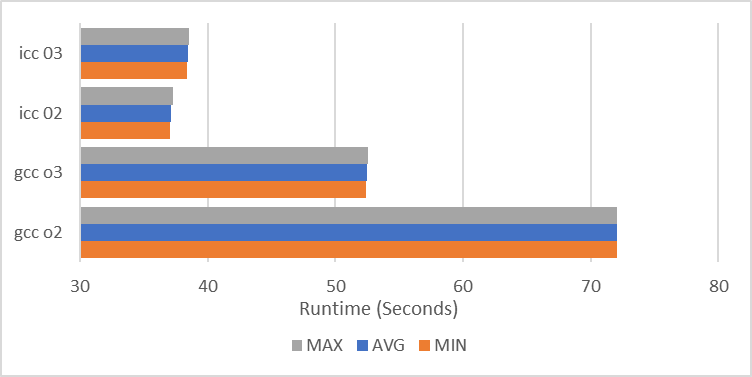
\includegraphics[width=0.8\linewidth]{figures/1-SEQ.png}
        \caption{Solve times achieved for $4000\times4000$ with the original serial code on various compilers. Min, Avg. and Max figures were taken from 10 repeated runs of the code.}
        \label{fig-1-seq}
\end{figure}

For this report, timings after different optimisations will be graphed for the different compilers and flags at $4000\times4000$. The fexact compilation command used through the report was simply \texttt{[gcc|icc] -std=c99 -Wall -O[2|3] -[q|f]openmp}. The choice of $4000\times4000$ strikes the best balance of having the ability to see how the algorithm performs due to spending a larger proportion of time on calculation with less run time variance from thread overhead. All graphs will include a minimum, average and maximum \textit{solution time} figure, taken from 10 execution repeats of the implementation at that point. It should also be noted that order to simplify the process of adding OpenMP pragma's later in the report, the serial code which used \texttt{static inline} functions was flattened into just one main computation function - something that had no performance hit. \par


%%%%%%%%%%%%%%%%%%%%%%%%%%%%%%%%%%%%%%%%%%%%%%%%%%%%%%%%%%%%%%%%%%%%%%%%%%%%%%%%
%%
\section{Approaching the Problem}
As was discovered previously, the majority of computation within the Jacobi method was calculating the matrix dot products. Currently in the serial method, this is within a double nested for loop. Each iteration of the outer loop is distinct, in that they require no dependency on other iteration's solutions in order to be computed. This makes the problem embarrassingly parallelisable as different iterations of the loop can be distributed amongst different workers. \par


%%%%%%%%%%%%%%%%%%%%%%%%%%%%%%%%%%%%%%%%%%%%%%%%%%%%%%%%%%%%%%%%%%%%%%%%%%%%%%%%
%%
\section{OpenMP and Optimisations}
Given the knowledge that this outer \texttt{for} loop is in fact embarrassingly parallelisable, OpenMP can be introduced very trivially. OpenMP is a API that allows for multiprocessing amongst different platforms and languages. Within the context of the code for this report - which is written in C - this is implemented with the addition of a compiler flag to enable OpenMP, and pragmas to control it. There are also some environment variables and API functions, however the majority of control comes from the aforementioned pragmas.

\subsection{Parallel For}
The first step in parallelising the code is to add one of the most fundamental and basic pragmas offered by OpenMP; \texttt{\#pragma omp parallel for}, which is inserted above the line declaring the outer for loop. The \texttt{parallel} keyword states that a team of threads should be created to execute the next control block in a parallel manner. The \texttt{for} keyword more specifically states that the iterations of the following loop should be run in the established team of threads. By default this creates as many threads as there are logical cores on the host machine, which in this case is 16. \par

As already stated, there is no dependence with the dot product operations meaning this is a seems to be a perfectly valid starting point. However, the convergence checking does require some inter-thread dependency. Thus the difference measure code was moved out of the for loop into it's own sequential loop that runs after the parallel for loop. This will be addressed in due course, but running the preceding solution greatly reduces the time this method takes; from upwards of 70 seconds in the sequential case of \texttt{gcc -o2} (Figure \ref{fig-1-seq}) to below 20 seconds in most cases for all the compilers (Figure \ref{fig-2-omp}). The 29 second run with \texttt{gcc -o2} appeares to be an outlier, but for integrity was not ommited. \par

\begin{figure}[h]
        \centering
        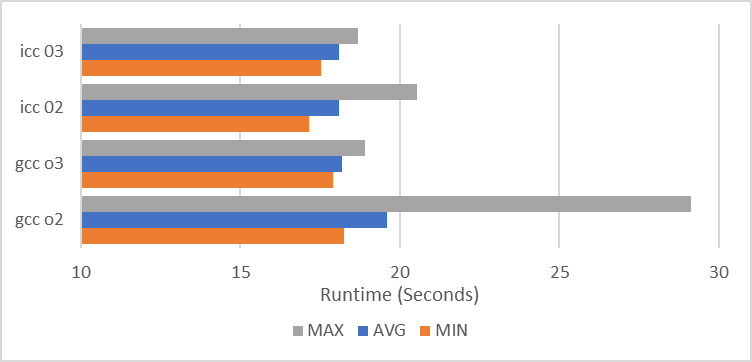
\includegraphics[width=0.8\linewidth]{figures/2-OMP-OUTER.png}
        \caption{Solve times achieved for $4000\times4000$ after adding the \texttt{\#pragma omp parallel for}.}
        \label{fig-2-omp}
\end{figure}


\subsection{Reduction}
In the last section, there was the slight hiccup of having to remove the difference measure from the main calculation loop. This leaves two loops, one for the main calculation and the other for calculating the difference measure. As the difference measure is far less computationally expensive, it could be left as it is. However, for the purpose of academic experimentation it would be beneficial to try and see if this can be improved upon. The first attempt carried out was to parallelise the second loop, however this has negligible difference and in many cases was slower. This can be attributed to the cost of initialising a team of threads more than required - in the first loop and then once again in the second loop. \par

With the failure of naive parallelism in this second loop, the \texttt{reduction} keyword was introduced to the original main loop pragma. OpenMP provides a \textit{'design pattern'} of sorts for the common problem of shared accumulators for teams of threads. This keyword instructs threads to do partial reduction operations on the chosen accumulator when they have completed running their work. These partial reductions eventually get collated into the final end value in a tree like fashion, dependant on the finish time of the thread. The thread's partial reductions are done with initial values that make sense to the reduction operation chosen (e.g. 0 for addition, 1 for multiplication), and not the user provided initial value for the accumulator - which in this case happens to be the same. This allows the threads to work privately and only collate the results later in execution time. \par

In the Jacobi implementation, the reduction is done with \texttt{+:sqdiff} and allows the two loops to be merged back together. This addition bears only very small difference to the timing results, once again most probably due to the simplistic computation. In theory this does help due to reducing the number of thread team creations. \par

\begin{figure}[h]
        \centering
        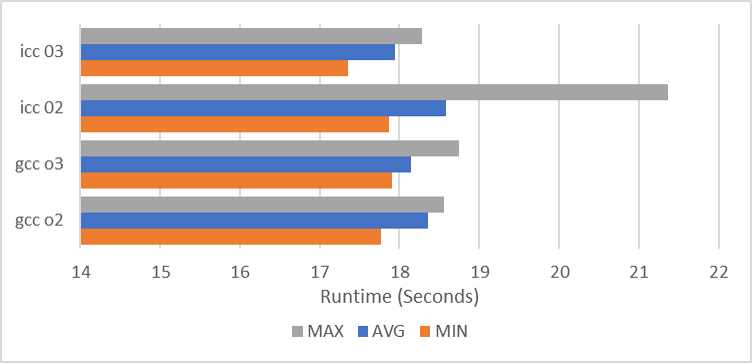
\includegraphics[width=0.8\linewidth]{figures/3-INNER-REDUX.png}
        \caption{Solve times achieved for $4000\times4000$ after introducing the \texttt{reduction} keyword for \texttt{sqdiff}.}
        \label{fig-3-redux}
\end{figure}


\subsection{Single Instruction, Multiple Data}
In the last report vectorisation was a prevalent topic. Not only were vectorisation options within the compiler explored, but also manual help was given in the form of explicitly calculating multiple rows at once to force a the processor to reduce cache invalidation. \par

OpenMP also adds support for single instruction, multiple data (SIMD) - i.e. vectorisation. This is a much more portable option as the implementation will deal with how the vectorisation is carried out within the compiler `optimally'. With this enabled, the very long, verbose \& explicit multiple row calculations were also removed from the implementation. This not only makes the code far more readable but also will fix any old bugs where problem sizes that are not divisible by 8 (the number of rows being calculated at once) would break for free. This had no tangible effect on the run time, meaning that OpenMP must be helping (inadvertently or not) helping mitigate cache invalidation. \par

\begin{figure}[h]
        \centering
        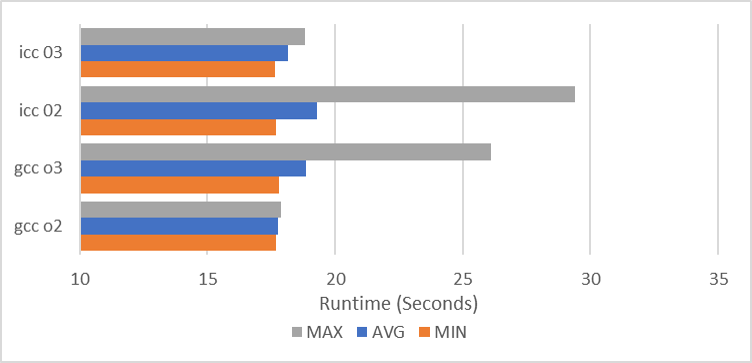
\includegraphics[width=0.8\linewidth]{figures/4-SIMD-W-REDUX.png}
        \caption{Solve times achieved for $4000\times4000$ after introducing the \texttt{simd} keyword in the main loop.}
        \label{fig-4-simd}
\end{figure}


%%%%%%%%%%%%%%%%%%%%%%%%%%%%%%%%%%%%%%%%%%%%%%%%%%%%%%%%%%%%%%%%%%%%%%%%%%%%%%%%
\section{Data Locality}
As with the sequential optimisations, great care must be taken into the usage of memory within high performance implementations. With the introduction of multiple physical cores, and multiple threads, there are now also multiple sources of memory to consider as well. \par

\subsection{Bluecrystal and NUMA}
For this report the implementation of the Jacobi method was run on The University of Bristol's ``Bluecrystal Phase 3" supercomputer. The individual node on which the code was tested has two Intel Sandy Bridge Xeon's in different sockets, with 8 cores in each, for a total of 16 logical cores. Each core has it's own Level 1 and 2 cache, and a shared Level 3 cache (per socket). The main memory is shared between the two CPU's, however certain portions of memory favour one processor or the other. The last notable piece of information about the host machine is the operating system, which in this case is a Linux system. \par

Linux operates a first touch policy on memory allocation, in that when memory is accessed for the first time by a process being run on the Linux Kernel, the data is put into a location in main memory. From this point on wards that data will always reside there unless programatically moved or copied. And due to the design of the nodes within Bluecrystal, and many other supercomputers, access times to main memory `belonging' to a different CPU is much slower than access to it's own memory. This problem is known as non-uniform memory access (NUMA), and this can have significant effects on run time. \par

When initialising the arrays for the Jacobi implementation, memory was previously allocated in a sequential loop. The compiler and kernel work to put this first touch of the memory next to the thread/core that initialised it. When moving to the now parallelised computational loop, this suddenly becomes problematic. This is because now the work is being distributed across \textit{all} the cores, and half of these will have much slower access to the memory as it assigned to the other CPU. \par


\subsection{Static Scheduling}
The solution for this problem is giving OpenMP a specific loop thread schedule. This is specified as an option to the \texttt{for} pragma; \texttt{schedule(kind)}, where \texttt{kind} can take the value of \texttt{static}, \texttt{dynamic}, \texttt{guided}, \texttt{auto} or \texttt{runtime}. The \texttt{static} scheduling kind was chosen as it provides deterministic allocation of threads to cores. \par

As this job is only run on one machine with equally powered cores, and the loop iterations are approximately equal in computational complexity \texttt{static} is a sensible choice. However in the case of problems that have varying loop run times, or implementations that will run on cores of different power a different schedule may perform better - such as guided. This is due to different threads finishing jobs at different times and potentially being left waiting. For example imagine a scenario where some cores run at double the performance to the other cores; if threads were to have iterations divvied up equally, then the fast cores will complete much sooner and spend wasted time doing nothing. Whereas in the case of a more dynamic scheduling method, this could be mitigated. \par

In the Jacobi code, the initialisation was parallelised in the same form (nested for loops with \texttt{\#prama omp parallel for schedule(static)}) as the main loop. This ensured that memory was being touched for the first time in the by the same cores that will be used in the main calculations. This resulted in significant speedup from just under 20 seconds previously to well under 12 seconds (Figure \ref{fig-5-numa}).

\begin{figure}[h]
        \centering
        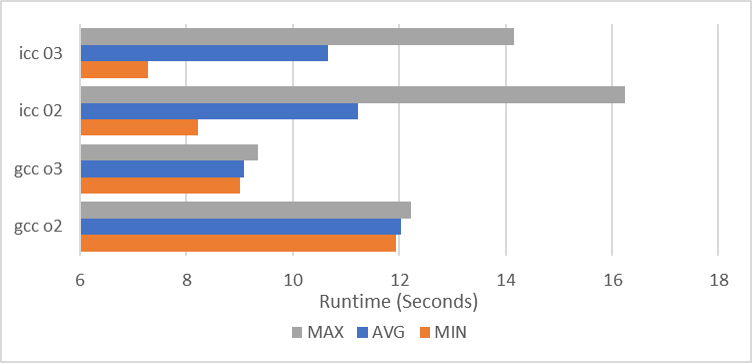
\includegraphics[width=0.8\linewidth]{figures/6-MEM-ALIGN-V2.png}
        \caption{Solve times achieved for $4000\times4000$ after mitigating NUMA by touching variables for the first time from appropriate cores.}
        \label{fig-5-numa}
\end{figure}


%%%%%%%%%%%%%%%%%%%%%%%%%%%%%%%%%%%%%%%%%%%%%%%%%%%%%%%%%%%%%%%%%%%%%%%%%%%%%%%%
\section{CPU Affinity}
Although there was a significant speedup in adding the static memory touching, now an extremely large variance in times is prevalent with the \texttt{icc} compiler had arisen. This is concerning, especially given that the solve times are far more consistent with the \texttt{gcc} compiler. However this very fact gives and indication that something programmatic is different between the compilers' outputs and that it is not some inherent property of the first-touch memory fixes. Having already looked at memory locality, the next obvious option is to look at which cores threads are being run on. \par

Before it was shown that it is possible to statically schedule iterations of the loops amongst threads, however there was no promise of threads \textit{actually} running on the same cores. OpenMP supports thread affinity options, which essentially dictates which core a given thread should run on. This is set with different environment variables, of which there are a few modes; \textit{Scatter} which will round robin threads through all of the different cores; \textit{Balanced} which tries to spread the threads in even ascending groups on the cores; and \textit{Close/Compact} which will try keep the threads as close together as possible. \par

Compact is useful for when trying to keep to the first socket on multi-socket machines, or where space locality is required. Scatter and Balanced perform almost identically if there are approximately as many threads as cores, but not if there are significantly more/less. Deciding whether to choose one or the other will depend on the problem and run configuration. If running with slightly more threads than cores on a socket, but less than the total number of cores, the balanced affinity will spread compute and memory resources. If running with more threads than cores, choosing balanced or scatter will depend on the memory alignment of the problem. \par

As benchmarks have been run with 16 cores, the affinity does not really matter. \texttt{ICC} defaults to no affinity, meaning the system decides. When the memory is being initialised the affinity decided by the system could be similar or completely different to that of the computational loop. In the cases of the affinities being similar, the results are closest to the optimal results gained when setting an affinity (Figure \ref{fig-6-affin}), but when they are not similar they are much more like the best results back  before NUMA mitigation was added (Figure \ref{fig-4-simd}). \par

\begin{figure}[h]
        \centering
        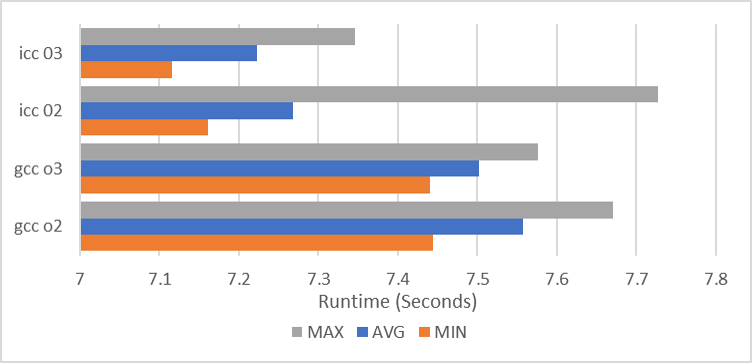
\includegraphics[width=0.8\linewidth]{figures/7-CPU-AFFIN.png}
        \caption{Solve times achieved for $4000\times4000$ after introducing compact CPU affinity.}
        \label{fig-6-affin}
\end{figure}

\small\textit{Upsettingly, documentation was too sparse/hidden for me to find the default affinity for \textit{GCC}. It clearly was doing something to help with affinity as the times were much more stable.}


%%%%%%%%%%%%%%%%%%%%%%%%%%%%%%%%%%%%%%%%%%%%%%%%%%%%%%%%%%%%%%%%%%%%%%%%%%%%%%%%
\section{Thread Scaling}
Having now looked at various aspects around parallelising the implementation, it is clear to see that the solve time has dramatically reduced by some 5-10 times, dependant on the compiler. The next of of note is looking at how the implementation performs with different numbers of threads, which is graphed below. Recall that the nodes this was run on have 16 logical cores.

\begin{figure}[h]
        \centering
        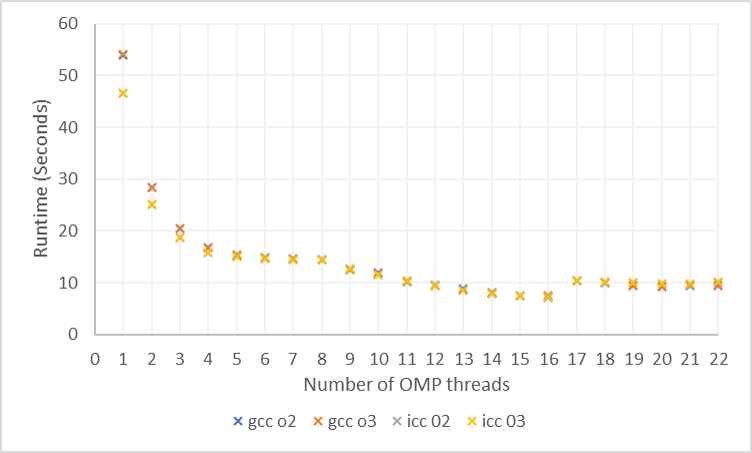
\includegraphics[width=0.8\linewidth]{figures/FINAL-THREAD-SCALING.png}
        \caption{Solve times achieved for $4000\times4000$ with different numbers of OpenMP threads using the compact affinity.}
        \label{fig-6-affin}
\end{figure}

This shows a few points of interest. Firstly, it is immediately apparent how quickly performance increases when there is under 8 threads. It follows an approximately exponential curve - something one would expect to see with the compact affinity. Then, the next small bump in speedup is when introducing the second socket and passing to more than 8 threads. However interestingly at this point the rewards reaped are much lower. Switching to a balanced affinity may have aided this, albeit possibly not that much. And then finally, when the number of threads surpasses the number of physical cores, the system relies on the kernel's time scheduler. This results in slightly slower, wavering, but roughly similar times even with scaling threads. \par

%%%%%%%%%%%%%%%%%%%%%%%%%%%%%%%%%%%%%%%%%%%%%%%%%%%%%%%%%%%%%%%%%%%%%%%%%%%%%%%%
\section{More Nodes; OpenMPI}
After exploring the possibilities with a single node performance one may ask, what now? Adding more nodes seems to be the obvious option. OpenMPI is a message passing library that allows for scaling parallel programs to multiple nodes within a high performance computing environment. An attempt was made at running OpenMPI within the implementation but ultimately ended in failure due to a very small bug that was sadly not fixed in time. This section serves as the motivation and planning regarding this attempt. \par

The main area of work that is distributed amongst the threads is the main for loop, so this is the target for distribution across multiple nodes. After initialising OpenMPI, each spawned node initialises the random data off of the fixed seed. Then they go straight into processing the main loop. The only cross node dependency is the array \texttt{X}, which stores the working and eventually final solutions to the Jacobi method. The motivation was to simply have all workers calculate their `chunk' of rows, synchronise this back to the master thread, and then have the fully updated array returned to them. The squared difference measure for measuring convergence was also passed around in it's partial form, in order to save extra processing. \par

In addition to the message passing to synchronise nodes from iteration to iteration, the plan was to keep the OpenMP implementation in place. This means that each node would calculate on it's section of the array in parallel, and then these would in turn synchronise back with OpenMPI. Sadly this did not come to fruition due to a small bug somewhere, presumably a finer detail overlooked within the maths. The message passing worked, the synchronisation appeared to work (perhaps some edge case of data was not being passed correctly, but the bulk was), and yet the figures for measuring convergence were wrong. This resulted in incorrect halting of execution and thus incorrect answers. Given another day to come back to this, the solution would likely be simple, but alas! \par


%%%%%%%%%%%%%%%%%%%%%%%%%%%%%%%%%%%%%%%%%%%%%%%%%%%%%%%%%%%%%%%%%%%%%%%%%%%%%%%%
\section{Conclusion}
In conclusion, this report ventured upon new ground from the original with the advent of parallelism. However, it is clear to see that similar areas cause the most dramatic decrease in solve times; management of memory is still crucial in order to maintain the best performance from one's code! The main critical addition to this is also thread location, which can almost be thought of in a similar fashion to memory. Locality is key, and ensuring efficient movement of memory, or communication between cores is vital! \par

After re-enabling the compiler flags from the serial assignment which added; floating point arithmetic optimisations; prefetch optimisations, intel's math-kernel library and other small tweaks, the final best times were achieved. These were approximately 0.2-0.3 seconds faster than the last fastest times in the CPU Affinity section (Figure \ref{fig-6-affin}). The final best times for this report are listed below: \par

\begin{table}[h]
\begin{adjustwidth}{-0.15cm}{}
\small
\centering
\begin{tabular}{c|c|c}
\textbf{Size} & \textbf{Solve Time (sec)} & \textbf{Compiler} \\ \hline
\textbf{500$\times$500}   & 0.185531 & \texttt{gcc -o2} \\
\textbf{1000$\times$1000} & 0.100523 & \texttt{icc -o3} \\
\textbf{2000$\times$2000} & 0.288259 & \texttt{icc -o3} \\
\textbf{4000$\times$4000} & 6.961660 & \texttt{icc -o3} \\
\textbf{8000$\times$8000} & 53.748440 & \texttt{icc -o3}

\end{tabular}
\caption{The final best times recorded from 10 runs of the implementation. Note that $500\times500$ performed poorly on \texttt{icc} and \texttt{gcc -o2} with fast floating point maths was used.}
\label{finalResults}
\end{adjustwidth}
\end{table}\par
\vspace{-0.22cm}

%%%%%%%%%%%%%%%%%%%%%%%%%%%%%%%%%%%%%%%%%%%%%%%%%%%%%%%%%%%%%%%%%%%%%%%%%%%%%%%%
%%  Bibliography
% \vspace{-0.3cm}
% \printbibliography[title={Bibliography}]
\end{document}

% \begin{figure}[h]
%     \includegraphics[width=18em]{Figures/twoLayers.pdf}
%     \centering
%     \caption{Two Layers to be composed together.}
%     \label{twolayers}
% \end{figure}
